\documentclass[letterpaper,10pt,conference]{ieeeconf}

\IEEEoverridecommandlockouts
\overrideIEEEmargins
\usepackage[utf8]{inputenc}
\usepackage[T1]{fontenc}
\usepackage{amsmath,amssymb,booktabs,graphicx,microtype}
\usepackage{cite}
\usepackage{xcolor}
\usepackage{hyperref}
\hypersetup{hidelinks}

\title{\LARGE \bf Decision-Level Auditing of Latent Robot World Models}
\author{Anikait Rana\textsuperscript{1}, Siddhant Rana\textsuperscript{1}, and Aditya Rao Udupi\textsuperscript{1}%
\thanks{\textsuperscript{1}Independent Researcher.}}

\begin{document}
\maketitle

\begin{abstract}
Latent world models are often judged by prediction error, but robot planning
depends on whether predicted futures rank candidate actions correctly. We introduce a
decision-level audit that separates these questions. On frozen 300-action
Push-T menus from released JEPA-WM and DINO-WM planners, we compare the action
chosen from predicted terminal latents ($P$) with the action chosen after
scoring simulator-realized endpoints in the same latent space ($O$). We evaluate
both choices using goal-distance utility $G$ (negative final-state distance) and
task reward $J$. Across 20 trajectory clusters and 562 model-matched rows,
predicted scoring substantially
outperformed uniform menu selection. Replacing predictions with realized
endpoints, however, did not reliably improve physical outcomes: the raw
$O$-versus-$P$ effect was $-5.30$ in $G$ (95\% CI $[-9.64,-0.71]$,
Holm-adjusted exact $p=.0755$) and $+0.042$ in $J$ ($[-0.176,0.240]$,
$p=.701$). Across all 577 merge-valid diagnostic artifacts, $P$ and $O$ selected
different actions in 337; only 48 and 38 of those switches reversed the strict
$G$-best and $J$-best pairwise ordering, respectively. The central result is a
separation: the latent scores were useful for choosing actions, but more faithful
terminal latents did not reliably make those choices better. A post-hoc,
prediction-only near-tie score nevertheless tracked these selector changes
(exploratory AUROC $.714$, 95\% trajectory-bootstrap CI $[.665,.762]$): the
held-out top ambiguity quarter switched $82.4\%$ of the time versus $51.0\%$
otherwise. It did not identify higher planner regret, so we treat it only as a
candidate trigger for prospective verification rather than call it physical
risk or epistemic uncertainty.
\end{abstract}

\section{Introduction}

World models matter to robot planning through the decisions they induce. A
planner can fail because its model predicts the wrong future, but it can also
fail because its learned representation assigns a low cost to a physically poor
outcome. Conversely, an imperfect predictor may still preserve the action
ordering needed for control. Standard prediction losses do not separate these
cases. Planning-oriented model learning and value equivalence formalize the
distinction
\cite{pmlr-v54-farahmand17a,pmlr-v120-lambert20a,pmlr-v119-nair20a,grimm2020value};
recent benchmarks measure world models through ranking and regret
\cite{reka2026worldmodelgym,pmlr-v267-yin25f}.

We ask a direct counterfactual question: \emph{if the same candidate actions are
scored using what actually happened in the simulator, does the planner choose a
better action?} For each candidate, we replace its predicted terminal latent
with an encoding of its realized endpoint. The action menu, encoder, latent
goal, cost function, and physical evaluation remain fixed. Any improvement is
therefore decision quality recovered by removing terminal prediction error from
the existing planning interface.

In plain terms, $P$ asks what the planner chooses from its prediction, $O$ asks
what it chooses after seeing the realized endpoint, and $G/J$ judge both selected
actions by their physical outcomes.

We make three contributions. First, we define a matched $P/O/G/J$ intervention
that connects latent prediction errors to action choice and physical regret.
Second, we derive exact candidate- and pair-level score accounting that explains
which prediction errors change a finite-menu decision without requiring semantic
coordinates or a global model of latent geometry. Third, we apply the audit to
released JEPA-WM and DINO-WM Push-T planners under a preregistered analysis. The
predicted scores contain useful action-selection signal, yet replacing predicted
endpoints with realized ones does not recover decision quality on average.
As a separate exploratory analysis, a selective diagnostic shows that the predicted
top-two margin can flag selector instability before simulator replay, while
failing to flag higher physical regret.

\begin{figure*}[t]
\centering
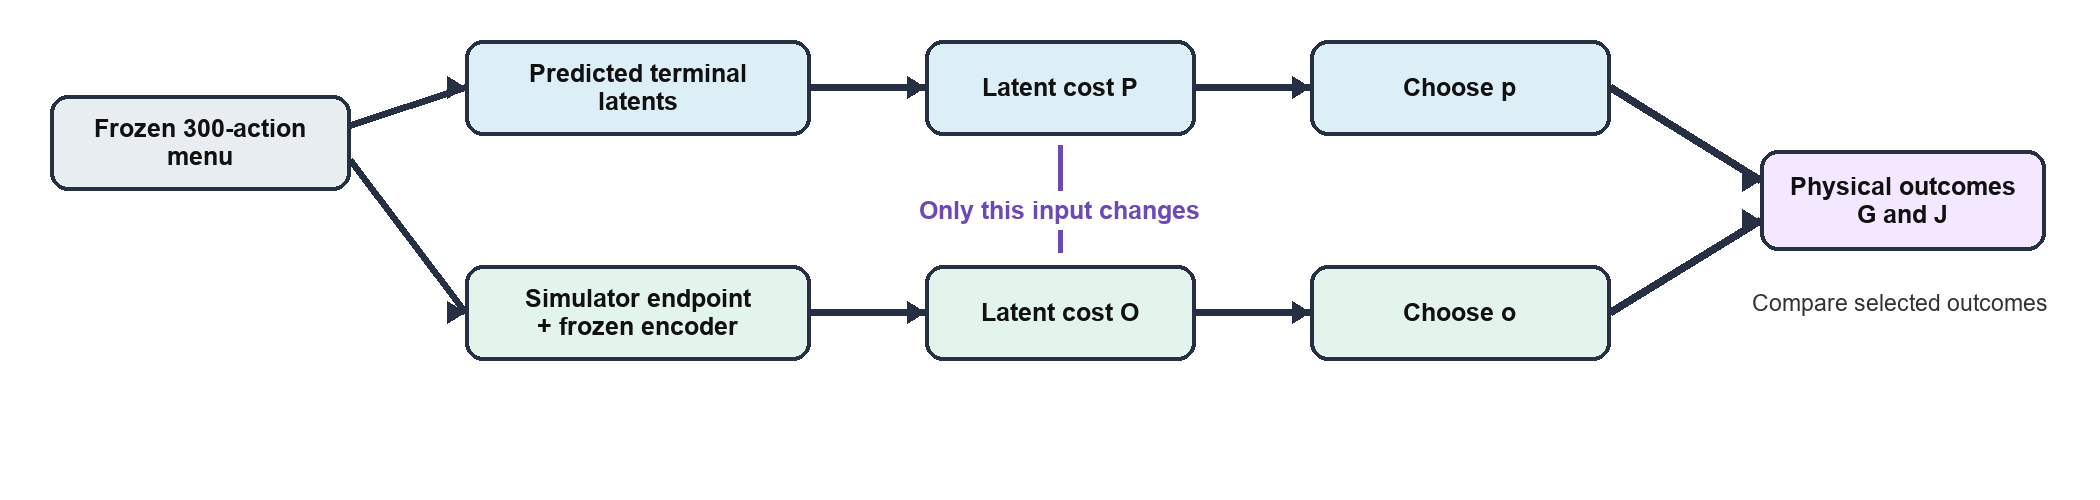
\includegraphics[width=0.96\textwidth]{audit_schematic.png}
\caption{Matched decision intervention. The candidate actions, encoder, goal
latent, and cost are fixed. Only the terminal state supplied to the latent cost
changes: model prediction for $P$, simulator-realized endpoint for $O$. Native
physical outcomes $G$ and $J$ evaluate the two selected actions.}
\label{fig:audit}
\end{figure*}

\section{Relation to prior evaluation}

Decision-aware model learning distinguishes predictive accuracy from the
quantities a downstream controller uses. Value-aware losses and value
equivalence formalize models that preserve decisions without reconstructing
every aspect of the environment
\cite{pmlr-v54-farahmand17a,pmlr-v120-lambert20a,grimm2020value}, while
goal-aware prediction emphasizes task-relevant features
\cite{pmlr-v119-nair20a}. Recent benchmarks likewise evaluate world models
through downstream ranking, regret, and control rather than reconstruction
alone \cite{reka2026worldmodelgym,pmlr-v267-yin25f}.

Robot world-model studies have also isolated objective and interface failures.
Latent objectives may discard information their planners need
\cite{singh2026objective}, and failures can remain hidden in aggregate offline
metrics \cite{vesessook2026hidden}. Our claim is narrower than proposing a new
loss or benchmark suite. Unlike decision-fidelity benchmarks that score a
model's downstream utility, our audit intervenes within a fixed planner: it
replaces only predicted terminal endpoints with their realized, re-encoded
counterparts, estimating the decision regret recoverable specifically from
terminal prediction correction. Unlike objective-swap studies, the
representation, objective, candidate set, and planner interface remain fixed.

\section{Matched decision intervention}

\subsection{Four views of the same action}

For action sequence $U_i$, let $\hat v_i,\hat r_i$ denote its predicted visual
and proprioceptive terminal latents, $v_i,r_i$ the corresponding latents after
simulator replay and frozen re-encoding, and $q_v,q_r$ the encoded goal. The
released lower-is-better costs are
\begin{equation}
\begin{aligned}
P_i&=\operatorname{MSE}(\hat v_i,q_v)
     +\alpha\operatorname{MSE}(\hat r_i,q_r),\\
O_i&=\operatorname{MSE}(v_i,q_v)
     +\alpha\operatorname{MSE}(r_i,q_r),
\end{aligned}
\label{eq:scores}
\end{equation}
with the released proprioceptive weight $\alpha=0.1$. $G_i$ is negative
official final simulator state distance to the dataset goal, and $J_i$ is the
float32 sum of the 30 official Push-T coverage rewards. Thus $P/O$ are
lower-is-better latent costs, whereas $G/J$ are higher-is-better physical
utilities. Crucially, $O$ is not a physical oracle: it supplies the true
endpoint to the same potentially misaligned learned encoder and latent
objective. With
$p=\arg\min_iP_i$, $o=\arg\min_iO_i$, and $Y\in\{G,J\}$, define
\begin{equation}
\Delta^Y = \bigl[\max_iY_i-Y_p\bigr]-\bigl[\max_iY_i-Y_o\bigr]=Y_o-Y_p.
\end{equation}
Positive $\Delta^Y$ favors $O$ over $P$. At the aggregate level, a non-positive
estimate indicates no average recovery under the unchanged interface.

This estimand is finite-menu and action-matched. Let
$R_s^Y=\max_iY_i-Y_s$ be the regret of selector $s\in\{p,o\}$. Then
$\Delta^Y=R_p^Y-R_o^Y$ measures regret removed by terminal prediction
correction, whereas $R_o^Y$ is regret that remains after correction. The latter
can arise from the representation, latent goal cost, terminal-only scoring, or
candidate support; the intervention does not identify those causes separately.

\subsection{Exact latent-score accounting}

For either latent block, let $q\in\mathbb{R}^d$ be the goal, $z_i$ the encoded
realized endpoint, and $\hat z_i=z_i+e_i$ its prediction. Expanding the square
gives
\begin{equation}
\begin{split}
P_i-O_i
&=d^{-1}\|\hat z_i-q\|_2^2-d^{-1}\|z_i-q\|_2^2\\
&=\underbrace{2d^{-1}(z_i-q)^\top e_i}_{D_i}
+\underbrace{d^{-1}\|e_i\|_2^2}_{M_i}.
\end{split}
\label{eq:decomp}
\end{equation}
$D_i$ is signed goal-directional error: it records whether error moves the
prediction toward or away from the latent goal. $M_i\geq0$ is error magnitude.
We compute both terms separately for visual and proprioceptive blocks and
combine them with the same $\alpha=0.1$ as Eq.~\ref{eq:scores}.
For candidates $a,b$, the change in their score margin is exact:
\begin{equation}
(P_a-P_b)-(O_a-O_b)=(D_a-D_b)+(M_a-M_b).
\label{eq:pair}
\end{equation}
Thus the audit can attribute a ranking reversal to directional or magnitude
terms without interpreting individual coordinates. This is local score
accounting, not a claim that the latent space is globally identifiable or
physically disentangled.

\subsection{What the intervention can establish}

Three outcomes are possible. If $P$ and $O$ agree, prediction error did not
change the selected action on that menu. If they disagree and $\Delta^Y>0$,
correction recovered some physical regret. If they disagree without positive
aggregate recovery, prediction error changed the planner's ranking but did not
provide evidence that it was a sufficient or dominant recoverable bottleneck
under the frozen representation and interface. The last case motivates
diagnosis of the remaining interface; it does not by itself prove which
component is faulty.

\section{Frozen Push-T study}

\subsection{Models, task, and candidate support}

We audit released JEPA-WM and DINO-WM Push-T checkpoints
\cite{terver2026drives,pmlr-v267-zhou25t}. Both use DINOv2 features, so this is
not a comparison of independent representation families. Each issued row holds
an outcome-blind common-initial menu of 300 six-step actions matching released
CEM initialization. Every action is replayed from the same state. The audit
covers iteration-0 menus, not later CEM populations or closed-loop control.

Push-T requires a planar agent to push a T-shaped block toward a target pose.
It is useful here because different short action sequences can look similar in
latent cost while producing different block displacement and task reward. For
each of 20 validation trajectories, the study samples five outcome-blind
offsets and three menu seeds for both predictors: $20\times5\times3\times2=600$
issued model rows. Candidate actions are identical across
the $P$, $O$, $G$, and $J$ views within a row, eliminating candidate-generation
changes as an explanation for a within-row selector difference.

\subsection{Frozen inference and validity rules}

Trajectories are the inferential units. A cell is one
trajectory--offset--seed combination containing both model rows. The frozen
analysis uses 20 trajectory clusters, a model-matched mask (562 valid model
rows; 281 matched cells), and a fixed 15-cell denominator per trajectory
($5$ offsets $\times3$ seeds). Within each cell, the two models receive equal
weight; cell effects are averaged within trajectory before inference. The
analysis uses deterministic
10,000-resample percentile bootstrap intervals, and exact trajectory-level
sign-flip tests (assuming sign symmetry). Holm correction is applied separately
within each preregistered two-outcome $G/J$ family for raw, bounded-$S$, and
$P$-versus-uniform analyses. Invalid or unmatched cells contribute zero
\emph{evidence} for both models in the fixed denominator, not a physical outcome
of zero. This fixed-denominator rule preserves equal scheduled exposure rather than
allowing whichever model completed more difficult cells to receive more
weight. The validity gate passed with 19/20 eligible trajectories.

The bounded support subset is defined before outcome analysis as
$S=\{U_i:\max|U_i^{\rm normalized}|\leq3\}$. It removes proposals at the
extreme tails of the normalized action distribution and re-runs the same
selector comparison on the remaining candidates. Exact duplicates are retained
in the inventory but deduplicated for strict winner selection; ambiguous
$P/O$ minima or negligible physical outcome ranges trigger abstention.

The primary recovery gate requires a positive $O$-versus-$P$ effect under the
preregistered trajectory-clustered test. A separate usefulness gate compares
$P$ against the exact expected outcome of uniformly sampling the same menus.
Standard menu-level ranking correlations, pairwise accuracies, normalized
regret, score decomposition, and model-specific summaries are descriptive:
they explain the primary result but do not create additional confirmatory
hypotheses.

\subsection{Post-hoc selective diagnostic}

After completing the preregistered analysis, we asked whether a planner could
identify decisions that deserve additional verification using predictions
alone. After collapsing physically duplicate actions, let $P_{(1)}$ and
$P_{(2)}$ be the two lowest predicted costs in a menu. We define
\begin{equation}
\begin{aligned}
m&=\frac{P_{(2)}-P_{(1)}}
        {\max(\operatorname{IQR}(P),10^{-12})},\\
U&=-\log_{10}\!\left(\max(m,10^{-12})\right),
\end{aligned}
\label{eq:ambiguity}
\end{equation}
so larger $U$ means a closer predicted race. This score uses no realized
latent or physical outcome. We evaluate it out of sample with
leave-one-trajectory-out (LOTO) logistic prediction of the event $p\ne o$,
including model identity as a baseline covariate. Each fold also sets a
model-specific top-quartile threshold using only its 19 training trajectories.
Uncertainty intervals resample whole trajectories 10,000 times. This analysis
is exploratory and was specified in a time-stamped post-hoc addendum before its
definitive run; it does not alter any preregistered test. The intervals condition
on the chosen score and fixed out-of-fold predictions; they neither account for
the earlier post-hoc choice of $U$ nor refit the full cross-fitting pipeline
inside each bootstrap resample.

\paragraph{Execution accounting.}
Of 600 issued model rows, 577 produced merge-valid artifacts and 23 remained
terminal-invalid; the stricter model-matched mask contained 562 rows (281
cells). Before outcome inspection, an outcome-blind infrastructure-recovery
amendment was applied without changing candidate menus or the frozen analysis.
Because this departed from the locked no-retry rule, we treat the evidence as
recovery-augmented and report an original-completions-only sensitivity below;
complete attempt-level provenance is preserved in a sealed audit package.

\section{Results}

\noindent\textbf{Headline separation.}
Confirmatory effects use the 562 model-matched rows, whereas switch-only
diagnostics use all 577 merge-valid artifacts. Predicted scoring beat uniform
selection, but realized-endpoint scoring did not reliably beat predicted
scoring. Thus, the score contained useful decision signal even though removing
terminal prediction error did not by itself recover better choices.

\begin{table*}[t]
  \caption{Trajectory-clustered physical effects. Positive favors the first
  named selector. Predictor-specific rows are descriptive because no
  model-interaction test was preregistered. $p_H$ denotes the Holm-adjusted
  exact sign-flip value.}
  \label{tab:effects}
  \centering
  \small
  \begin{tabular}{lcc}
    \toprule
    Contrast & $\Delta^G$ [95\% CI]; $p_H$ & $\Delta^J$ [95\% CI]; $p_H$ \\
    \midrule
    $O$ vs. $P$ (raw) & $-5.30$ [$-9.64,-0.71$]; $.0755$ & $0.042$ [$-0.176,0.240$]; $.701$ \\
    $O$ vs. $P$ (bounded) & $-5.80$ [$-11.00,-0.21$]; $.111$ & $0.115$ [$-0.093,0.314$]; $.296$ \\
    $P$ vs. uniform & $48.70$ [$40.47,56.43$]; $7.63\!\times\!10^{-6}$ & $0.761$ [$0.420,1.117$]; $4.02\!\times\!10^{-4}$ \\
    \midrule
    DINO-WM: $O$ vs. $P$ (raw) & $-1.27$ [$-7.84,6.34$]; -- & $0.003$ [$-0.243,0.240$]; -- \\
    JEPA-WM: $O$ vs. $P$ (raw) & $-9.33$ [$-14.61,-4.67$]; -- & $0.081$ [$-0.135,0.279$]; -- \\
    \bottomrule
  \end{tabular}
\end{table*}

\paragraph{Latent scoring contains action-selection signal.}
$P$ exceeded the exact expected physical outcome of uniformly sampling the same
candidate menus by $48.70$
in $G$ (95\% CI $[40.47,56.43]$, adjusted $p=7.63\times10^{-6}$) and $0.761$
in $J$ ($[0.420,1.117]$, $p=4.02\times10^{-4}$). Both outcomes passed the
preregistered usefulness gate.

\paragraph{Realized endpoints do not reliably improve selection.}
The raw $P\!\rightarrow\!O$ physical-outcome effect was $-5.30$ in $G$
($[-9.64,-0.71]$, adjusted $p=.0755$)
and $+0.042$ in $J$ ($[-0.176,0.240]$, $p=.701$). Bounded-$S$ estimates had the
same qualitative pattern:
$-5.80$ in $G$ ($[-11.00,-0.21]$, $p=.111$) and $+0.115$ in $J$
($[-0.093,0.314]$, $p=.296$). Although both marginal bootstrap intervals for
$G$ excluded zero, neither Holm-adjusted exact test passed $\alpha=.05$. Under
the preregistered rule, the evidence does not support physical recovery. The
interval and adjusted $p$-value are not contradictory: the percentile interval
summarizes one marginal effect, whereas the Holm-adjusted exact test is the
preregistered multiple-testing decision rule; the two need not cross their
thresholds together.
The $G$ point estimate is 10.9\% of the $48.70$ predicted-versus-uniform
advantage in magnitude, in the same simulator state-distance units.
Descriptively, JEPA-WM accounts for most of the aggregate $G$ difference
($-9.33$, versus $-1.27$ for DINO-WM); no model-interaction test was
preregistered, so this split is hypothesis-generating rather than confirmatory.

\begin{figure*}[t]
\centering
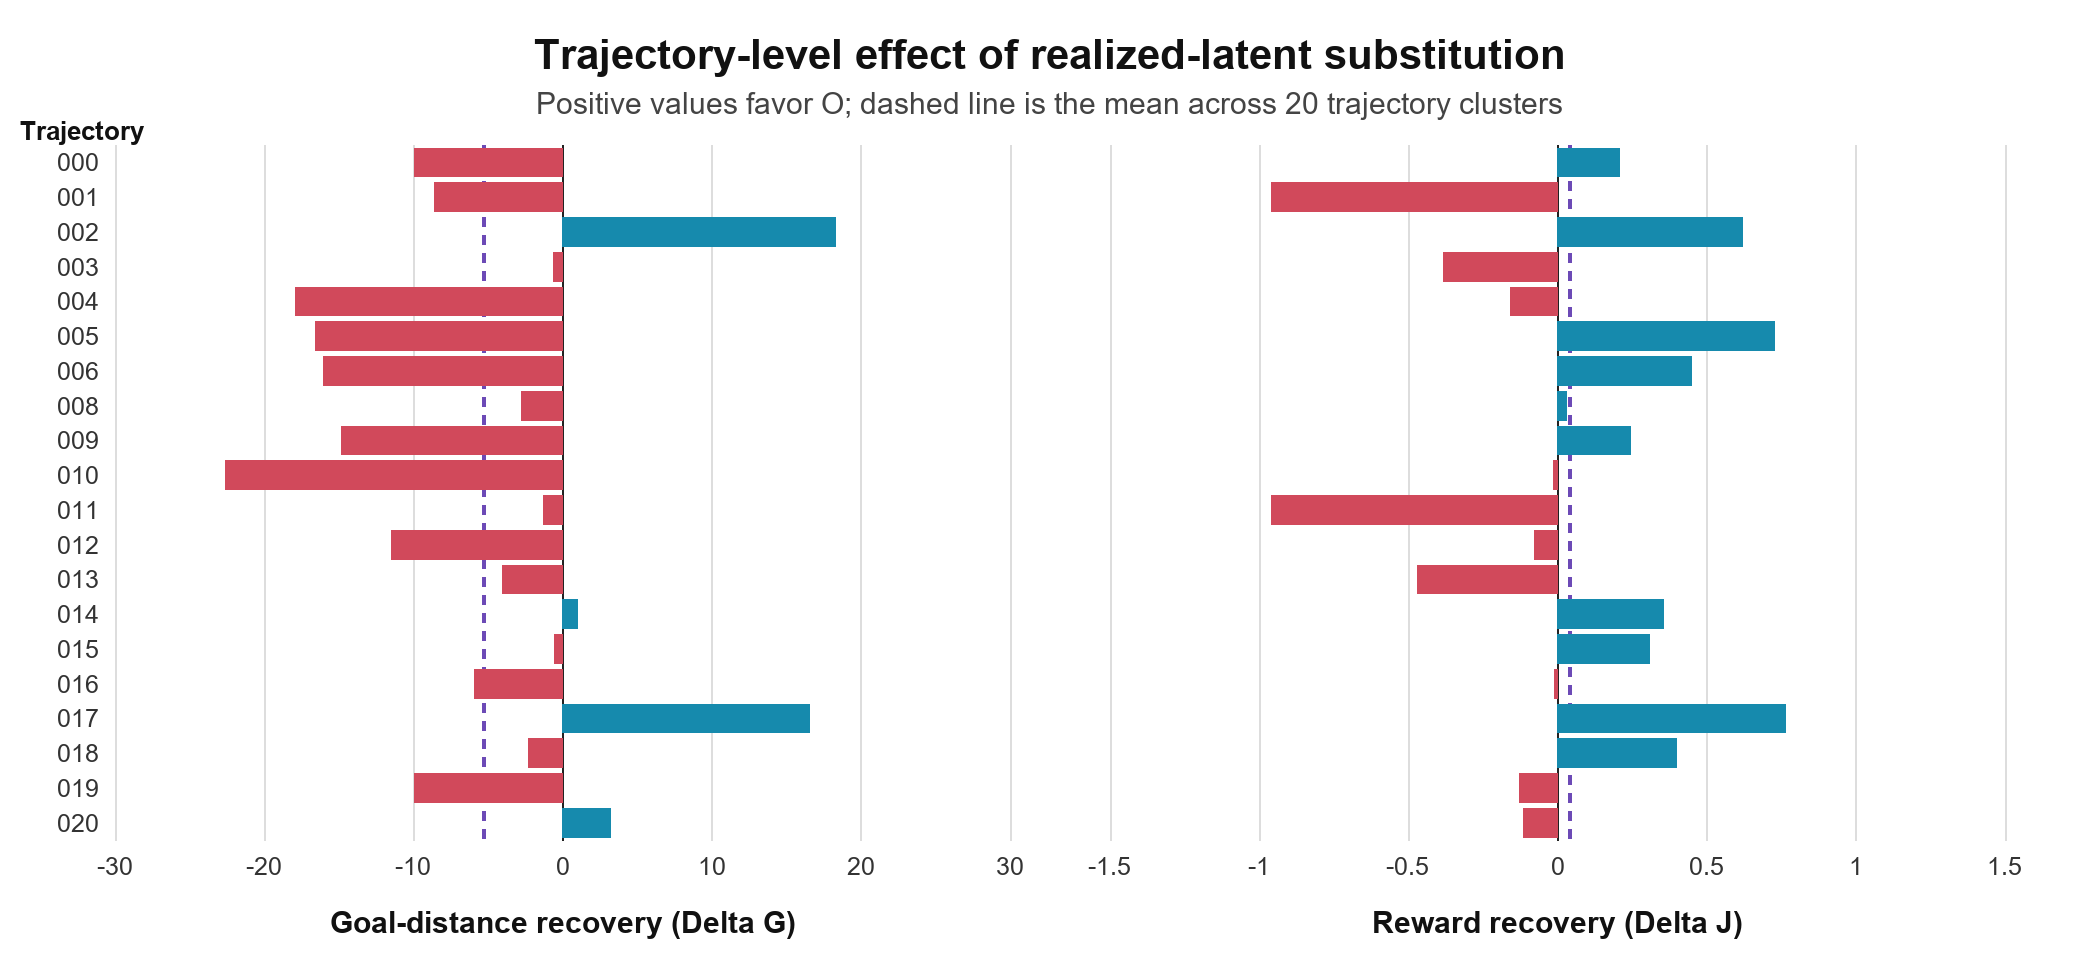
\includegraphics[width=0.94\textwidth]{trajectory_effects.png}
\caption{The primary effect resolved by inferential unit. Realized-latent
substitution improves goal distance on four of 20 trajectory clusters and
reward on ten, but the magnitudes are heterogeneous. The dashed line is the
unweighted cluster mean used in the raw analysis; this display is descriptive
and does not replace the preregistered exact tests. All 20 scheduled clusters
remain in the fixed-denominator estimate; eligibility is a validity threshold,
not an exclusion rule.}
\label{fig:clusters}
\end{figure*}

Most $G$ cluster effects in Figure~\ref{fig:clusters} are negative, with two
large positive exceptions; $J$ improvements and degradations are nearly
balanced. This heterogeneity supports trajectory-level inference and argues
against treating 562 model rows as independent samples.

\paragraph{Original-completions-only sensitivity.}
As an exploratory check, we discarded every recovery-sourced artifact and
reapplied the same fixed 15-cell matched aggregation. The remaining 408 matched
rows yielded $\Delta^G=-5.39$ ($[-9.32,-1.40]$) and
$\Delta^J=-0.019$ ($[-0.212,0.160]$); bounded-$S$ estimates were $-6.30$ and
$0.052$. Only 14 trajectories met the original eligibility threshold, so this
subset fails the locked validity gate and is not confirmatory. Its similar
scale and the same substantive non-recovery conclusion suggest that the headline
is not created by including the recovered rows.

\paragraph{Post-hoc latent interpolation.}
To test whether full endpoint substitution created an isolated selector artifact,
we scored stored interpolants
$\hat z_\lambda=(1-\lambda)\hat z+\lambda z$ for
$\lambda\in\{0,.1,\ldots,1\}$ without new simulator rollouts. At $\lambda=.5$,
38.4\% of selectors had changed and $\Delta^G=-2.24$; at $\lambda=1$, these
values were 58.9\% and $-5.30$. All ten nonzero-$\lambda$ $\Delta^G$ estimates
were negative, with a lambda--effect correlation of $-.946$; the endpoint was
also negative for each model and in the original-completions-only sensitivity.
Reward showed no graded trend ($r=.245$). This aggregate pattern argues against
the full-$O$ endpoint alone creating the result, but interpolated latents need
not correspond to realizable states and the analysis is explicitly post-hoc.

\paragraph{Correction frequently reranks actions, but seldom recovers the
oracle-best pair.}
Across 577 merge-valid diagnostic artifacts, $P$ and $O$ selected different
candidates in 337 rows (58.4\%). Among those disagreements, 48 (14.2\%), 38
(11.3\%), and 11 (3.3\%) produced recovery-aligned reversals of the strict
$P$-versus-$G$-best, $J$-best, and both pairs, respectively. These pair
counts deliberately cover only switches involving the strict oracle-best
candidate; they are a diagnostic complement to the aggregate recovery test.

\paragraph{Prediction-only near ties flag selector instability.}
On the 562 model-matched rows, $U$ had exploratory AUROC $.714$ for $P/O$
selector changes (trajectory-bootstrap 95\% CI $[.665,.762]$). The fitted LOTO
probability model had AUROC $.706$.
The training-fold-defined ambiguity quarter covered $25.3\%$ of held-out rows
and had $82.4\%$ switch risk, compared with $51.0\%$ elsewhere (risk ratio
$1.62$, $[1.44,1.82]$). Point estimates remained above chance for DINO-WM
(AUROC $.691$), JEPA-WM ($.734$), the bounded action set ($.696$), original
completions only ($.709$; 408 rows across 15 observed trajectories), and all
merge-valid artifacts ($.714$). The LOTO probability model improved
Brier score from $.243$ using model identity alone to $.214$ with $U$
(bootstrap difference $[-.043,-.016]$); raw and IQR-normalized margins were not
reliably different.

\begin{figure*}[t]
\centering
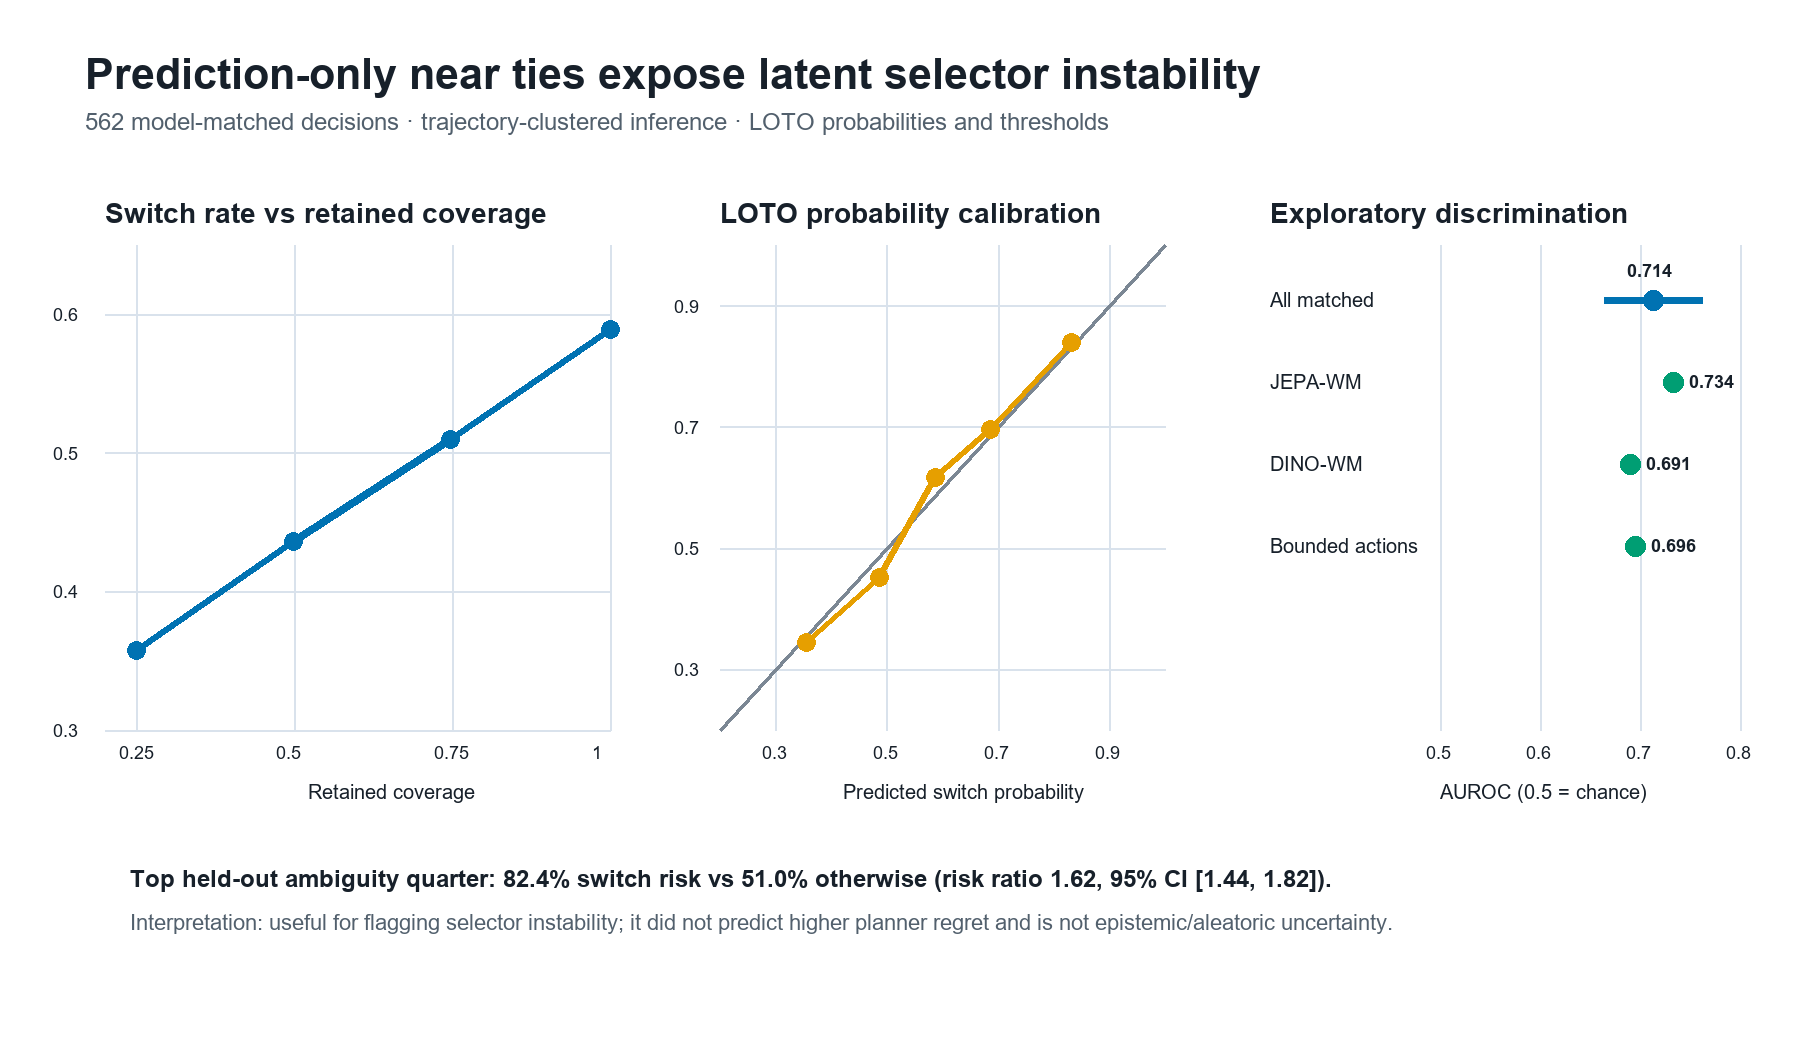
\includegraphics[width=.88\textwidth]{near_tie_instability.png}
\caption{Exploratory held-out selective
diagnostic. Retaining increasingly ambiguous decisions raises the $P/O$ switch
rate (left); descriptive LOTO calibration is shown in the middle;
discrimination point estimates remain above chance across both predictors and
bounded actions (right). The near-tie signal predicts selector instability,
not physical decision quality.}
\label{fig:near-tie}
\end{figure*}

Crucially, this is not a planner-regret result. The flagged-minus-unflagged
normalized regret was $-.007$ for $G$ (95\% CI $[-.039,.026]$) and $-.056$ for
$J$ ($[-.143,.026]$). Near ties reveal that the selected index is sensitive to
terminal prediction correction, but do not show that the deployed $P$ action
is physically worse. The score is therefore only a candidate signal for testing
a future verification policy; no control, safety, or cost-benefit improvement
was evaluated here.

\begin{table}[t]
  \caption{Descriptive menu-level ranking diagnostics on the preregistered
  bounded support $S$, averaged over valid rows. Higher is better for Spearman
  and pairwise accuracy; lower is better for normalized regret@1.}
  \label{tab:ranking}
  \centering
  \scriptsize
  \begin{tabular}{llrr}
    \toprule
    Physical outcome & Diagnostic & Predicted $P$ & Realized $O$ \\
    \midrule
    Goal distance $G$ & Spearman rank correlation & .367 & .345 \\
                      & Pairwise ranking accuracy & .599 & .591 \\
                      & Normalized regret@1 & .250 & .274 \\
    \addlinespace
    Reward $J$        & Spearman rank correlation & .121 & .124 \\
                      & Pairwise ranking accuracy & .469 & .471 \\
                      & Normalized regret@1 & .372 & .359 \\
    \bottomrule
  \end{tabular}
\end{table}

\paragraph{Prediction correction does not repair global ranking fidelity.}
The aggregate result is also visible beyond the selected top action.
Substituting $O$ for $P$ slightly reduces both goal-distance ranking measures
and increases normalized $G$ regret@1. Reward ranking is essentially unchanged,
with small improvements in pairwise accuracy, correlation, and regret@1.
Therefore the absent physical recovery is not merely an argmin anomaly: under
this fixed latent objective, more faithful terminal inputs do not consistently
produce a more physically faithful ordering of the 300 candidates.
Candidate support was not empty: the descriptive
\emph{oracle-within-top-$k$} upper bound, which uses outcomes and is not an
executable selector, reduced normalized regret from $.250$ to $.101$ for $G$
and from $.372$ to $.224$ for $J$ when $k=5$; $k=10$ reduced it further to
$.064$ and $.179$. The predictor often placed useful actions near the top
without reliably identifying the best one.

\paragraph{The exact decomposition audits score changes, not physical causes.}
Equation~\ref{eq:decomp} reconstructed $P-O$ to numerical precision (maximum
identity residual $6.66\times10^{-16}$). Directional terms dominated magnitude
terms in 266 of the 337 selector switches (78.9\%), but this label frequency was
nearly unrelated to trajectory-level recovery. The decomposition can therefore
identify which algebraic term flips a latent ranking; in this study it does not
establish a stable physical failure mechanism.

\section{Discussion}

\paragraph{Central finding.}
Taken together, the results reveal a gap between useful latent scores and
physically aligned decisions. Predicted scoring was substantially better than
uniform selection, so the planning signal was not arbitrary. Yet scoring the
realized endpoints changed more than half of the selected actions without
producing reliable aggregate physical improvement. Under these frozen menus and
the unchanged scoring interface, we therefore find no evidence that terminal
prediction correction is sufficient to recover decision quality. Possible
remaining sources include the representation, latent goal objective,
terminal-only scoring, and candidate support. Related work studies these design
choices directly \cite{singh2026objective,vesessook2026hidden}; our contribution
is a matched intervention that measures their combined consequence at the
decision boundary.

\paragraph{Using the audit as a diagnostic tool.}
The audit is designed for a released planner rather than a particular training
algorithm. It produces five linked outputs: (i) $P/O$ selector agreement,
(ii) native regret recovered or added by a switch, (iii) whole-menu ranking
fidelity, (iv) strict oracle-pair reversals, and (v) exact $D/M$ attribution of
the latent score change. Together these distinguish ``the prediction changed''
from ``the ranking changed'' and ``the physical choice improved.'' A practitioner
can run the same trace before retraining: strong $O$-over-$P$ recovery implicates
terminal prediction error as a recoverable bottleneck, while persistent $O$
regret directs attention to the objective, representation, temporal score, or
proposal set. That routing is diagnostic, not causal identification; the latter
requires a second intervention on the suspected component.

The post-hoc near-tie result adds an online-facing output to this offline audit.
A planner can compute $U$ from its existing predicted costs. Our result motivates
testing whether using it to route ambiguous menus to a more expensive verifier,
fallback, or human improves utility. Because $U$ did not identify higher
physical regret, this paper does not claim that such routing improves control,
safety, or cost-benefit tradeoffs.

\section{Limitations and reproducibility}

The study is limited to one simulated task and 20 independent trajectory
clusters. Its two predictors share DINOv2 visual features, so the descriptive
model split cannot support a general JEPA-versus-DINO conclusion. The audit
uses six model actions (five simulator steps each), terminal-only scoring, and
iteration-0 300-action menus rather than the released planner's complete
30-iteration CEM or closed-loop execution. A finite menu can also hide recovery
when it contains no materially better candidate, although the top-$k$ regret
results show that better actions were commonly present near the predicted top.

$O$ uses simulator-privileged endpoints and is an evaluation intervention, not
an online policy. The fixed-denominator rule avoids differential model exposure
but shrinks missing cells toward zero; because that shrinkage can favor a
non-recovery conclusion, the original-completions-only sensitivity is reported
separately. Failures correlated with decision difficulty could still affect the
estimand. No independent
replication was run. The selective analysis was designed after observing the
main non-recovery result and must be treated as hypothesis-generating despite
LOTO evaluation and trajectory-level intervals. Upon acceptance, we will
release an anonymized audit package containing the frozen manifest,
preregistration, recovery addendum, issuance and attempt ledgers, merge index,
sealed result, analysis code, and deterministic figure inputs. The 241-GB
per-row arrays are not duplicated
in that package; their paths and cryptographic bindings remain in the manifest
and merge index for full reconstruction from the retained evidence.

\section{Conclusion}

On Push-T, the audited latent scores selected better actions than a uniform
baseline, but replacing predicted endpoints with realized endpoints did not
yield statistically reliable physical improvement. The same correction changed
58.4\% of selections while leaving whole-menu physical ranking fidelity nearly
unchanged. These results illustrate why evaluating a world model for planning
requires more than measuring prediction error: the relevant question is whether
predicted futures preserve the action rankings that matter physically. The
$P/O/G/J$ audit turns that question into a matched, reproducible test without
retraining the model. A prediction-only near-tie score can additionally triage
which choices are likely to change under endpoint correction, but a separate
physical-risk signal is needed before such triage can promise better control.

\bibliographystyle{IEEEtran}
\bibliography{references}

\end{document}
